\let\lesson\undefined
\newcommand{\lesson}{\phantomlesson{Bài 2: Nhiệt độ. Thang nhiệt độ}}
\chapter[Nhiệt độ. Thang nhiệt độ.]{Nhiệt độ. Thang nhiệt độ.}
\section{Lý thuyết}
\subsection{Chiều truyền năng lượng nhiệt giữa hai vật chênh lệch nhiệt độ tiếp xúc nhau}
Khi cho hai vật chênh lệch nhiệt độ tiếp xúc nhau, năng lượng nhiệt luôn truyền từ vật có nhiệt độ cao hơn sang vật có nhiệt độ thấp hơn. Quá trình truyền nhiệt kết thúc khi hai vật ở cùng nhiệt độ (trạng thái cân bằng nhiệt).
\begin{center}
	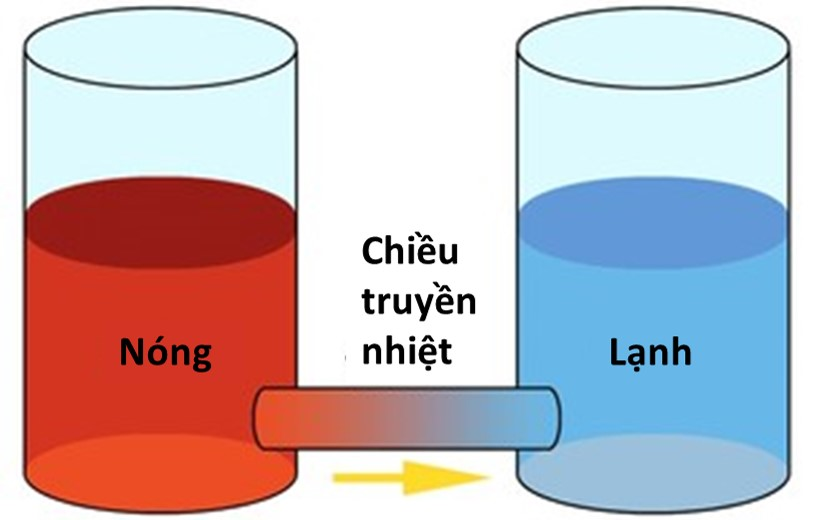
\includegraphics[width=0.3\linewidth]{../figs/VN12-Y24-PH-SYL-002-1}
	\captionof{figure}{Minh hoạ chiều truyền nhiệt giữa hai vật có nhiệt độ khác nhau.}
\end{center}
\subsection{Nhiệt độ}
\subsubsection{Khái niệm về nhiệt độ}
Nhiệt độ của một vật là đại lượng vật lí đặc trưng cho mức độ chuyển động nhiệt của phân tử vật chất cấu tạo nên vật. Khi các phân tử chuyển động nhiệt càng nhanh thì nhiệt độ của vật càng cao và ngược lại.
\subsubsection{Nhiệt kế}
Nhiệt độ đo trên nhiệt kế được xác định thông qua giá trị của một đại lượng vật lí khác mà đại lượng này phụ thuộc theo nhiệt độ.\\
\textbf{\textit{Ví dụ:}}
\begin{itemize}
	\item Nhiệt kế thuỷ ngân xác định nhiệt độ dựa trên hiện tượng dãn nở vì nhiệt của thuỷ ngân.
	\item Nhiệt kế điện trở xác định nhiệt độ qua sự phụ thuộc của điện trở theo nhiệt độ.
\end{itemize}
\begin{center}
	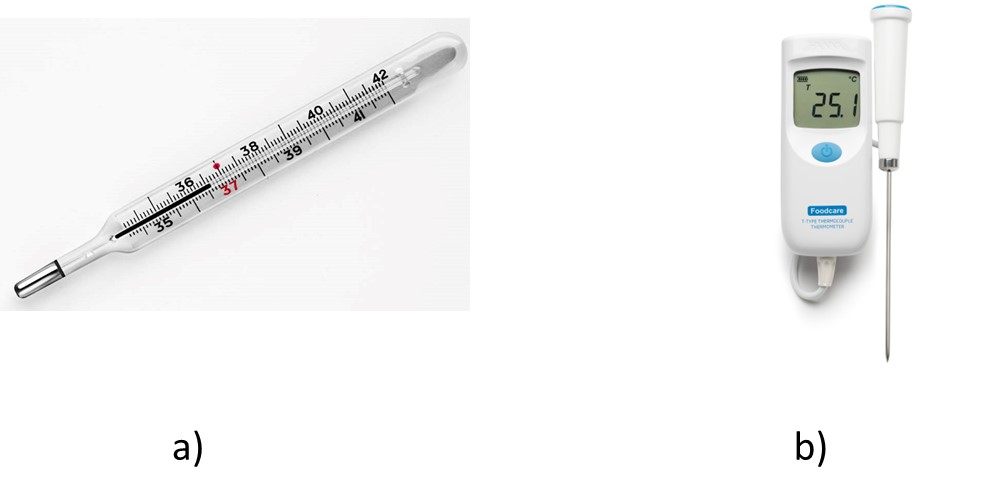
\includegraphics[width=0.5\linewidth]{../figs/VN12-Y24-PH-SYL-002-2}
	\captionof{figure}{a) Nhiệt kế thuỷ ngân; b) Nhiệt kế điện trở.}
\end{center}
\subsection{Thang nhiệt độ}
\subsubsection{Thang nhiệt độ Celsius}
Nhiệt độ trong thang đo này được kí hiệu là $t$. Đơn vị là độ Celsius (kí hiệu: $\si{\celsius}$).\\
$\SI{1}{\celsius}=\dfrac{1}{100}$ của khoảng cách giữa nhiệt độ nóng chảy của nước tinh khiết đóng băng $\left(\SI{0}{\celsius}\right)$ và nhiệt độ sôi của nước tinh khiết ở áp suất $\SI{1}{atm}$ ($\SI{100}{\celsius}$).

\subsubsection{Thang nhiệt độ Kelvin}
Nhiệt độ trong thang đo này được kí hiệu là $T$. Đơn vị là độ Kelvin (kí hiệu: $\si{\kelvin}$).\\
$\SI{1}{\kelvin}=\dfrac{1}{273,15}$ của khoảng cách giữa nhiệt độ không tuyệt đối $\left(\SI{0}{\kelvin}\right)$ và nhiệt độ điểm mà nước tinh khiết tồn tại đồng thời ở thể rắn, lỏng và hơi ở áp suất $\SI{1}{atm}$ ($\SI{273.15}{\kelvin}$).\\
Nhiệt độ không tuyệt đối ($\SI{0}{\kelvin}$) là nhiệt độ mà tại đó động năng chuyển động nhiệt của các phân tử cấu tạo nên vật chất bằng không và thế năng của chúng là tối thiểu.
\luuy{Một độ chia trên thang nhiệt độ Kelvin bằng một độ chia trên thang nhiệt độ Celsius.}
\subsubsection{Chuyển đổi nhiệt độ đo theo thang Celsius sang nhiệt độ đo theo thang Kelvin}
\begin{equation}
	T=t+273,15\approx t+273
\end{equation}
với:
\begin{itemize}
	\item $t$: giá trị nhiệt độ của vật theo thang nhiệt độ Celsius;
	\item $T$: giá trị nhiệt độ của vật theo thang nhiệt độ Kelvin.
\end{itemize}
\section{Mục tiêu bài học - Ví dụ minh hoạ}
\begin{dang}{Chuyển đổi được nhiệt độ đo theo thang Celsius sang nhiệt độ đo theo thang Kelvin và ngược lại.}
	\viduii{1}
	{Nhiệt độ của khối khí trong phòng đo được là $\SI{27}{\celsius}$. Xác định nhiệt độ của khối khí trong thang nhiệt độ Kelvin.
	
}
{\hide{
Nhiệt độ khối khí trong thang nhiệt độ Kelvin:
$$T=t+273=\SI{300}{\kelvin}.$$}

}

\viduii{2}
{Một nhiệt kế dùng để đo nhiệt độ của các lò nung có phạm vi đo từ $\SI{263}{\kelvin}$ đến $\SI{1273}{\kelvin}$.
	\begin{enumerate}[label=\alph*)]
		\item Xác định phạm vi đo của nhiệt kế này trong thang nhiệt độ Celsius?
		\item Nếu sử dụng nhiệt kế này để đo nhiệt độ lò nung đang nấu chảy đồng có nhiệt độ nóng chảy là $\SI{1083}{\celsius}$ thì nhiệt kế có đo được không? Vì sao? Em có khuyến cáo gì về việc sử dụng nhiệt kế trong tình huống này?
	\end{enumerate}

}
{\hide{
\begin{enumerate}[label=\alph*)]
	\item $t_\text{min}=T_\text{min}-273=\SI{-10}{\celsius};\quad t_\text{max}=T_\text{max}-273=\SI{1000}{\celsius}.$\\
	Phạm vi đo của nhiệt kế này trong thang nhiệt độ Celsius là $\SI{-10}{\celsius}$ đến $\SI{1000}{\celsius}$.
	\item Nếu sử dụng nhiệt kế này để đo nhiệt độ lò nung đang nấu chảy đồng có nhiệt độ nóng chảy $\SI{1083}{\celsius}$ thì nhiệt kế không đo được vì nhiệt độ cần đo nằm khoảng phạm vi đo của nhiệt kế.\\
	Trong trường hợp này, người đo cần dùng nhiệt kế có thang đo lớn hơn $\SI{1083}{\celsius}$ như nhiệt kế điện trở.
\end{enumerate}}
}
	
	\viduii{3}
	{Trong thang nhiệt độ Fahrenheit, chọn nhiệt độ tại điểm nước đá đang tan là $\SI{32}{\degree F}$, nhiệt độ tại điểm nước sôi ở điều kiện thường $\left(\SI{1}{atm}\right)$ là $\SI{212}{\degree F}$, trong khoảng nhiệt độ này chia thành 180 khoảng bằng nhau, mỗi khoảng ứng với $\SI{1}{\degree F}$. Thang đo này được nhà vật lí người Đức Daniel Gabriel Fahrenheit đề xuất vào năm 1724 và được sử dụng phổ biến ở các nước phương Tây. Nếu gọi $t$ là nhiệt độ của vật trong thang nhiệt độ Celsius và $T_\text{F}$ nhiệt độ của vật trong thang nhiệt độ Fahrenheit thì:
		$$T_\text{F}=a\cdot t+b.$$
		với $a$ và $b$ là các hệ số tỉ lệ.
		\begin{enumerate}[label=\alph*)]
			\item Em hãy xác định xác giá trị của $a$ và $b$.
			\item Trên tin tức thông báo nhiệt độ tại New York ngày 17/03/2024 là $\SI{49}{\degree F}$. Trong thang Celsius thì nhiệt độ này là bao nhiêu $\si{\celsius}$?
		\end{enumerate}
	
}
{\hide{
\begin{enumerate}[label=\alph*)]
	\item Nhiệt độ tại điểm nước đá đang tan là $\SI{32}{\degree F}$ hay $\SI{0}{\celsius}$:
	\begin{equation}
		\label{eq: 1}\\
		b=\SI{32}{\degree F}
	\end{equation}
Nhiệt độ tại điểm nước sôi ở điều kiện thường $\left(\SI{1}{atm}\right)$ là $\SI{212}{\degree F}$ hay $\SI{100}{\celsius}$:
\begin{equation}
	\label{eq: 2}\\
	212=100a+b
\end{equation}
Từ (\ref{eq: 1}) và (\ref{eq: 2}), suy ra:
\begin{equation*}
	\begin{cases}
		b=\SI{32}{\degree F}\\
		a=\SI{1.8}{\degree F/\celsius}
	\end{cases}
\end{equation*}
Như vậy, $T_\text{F}=1,8\cdot t+32.$
\item Nhiệt độ tại New York ngày 17/03/2024 theo thang Celsius:
$$t=\dfrac{T_\text{F}-32}{1,8}\approx\SI{9.44}{\celsius}.$$
\end{enumerate}}
}
\manatip{$$\dfrac{t\left(\si{\degree F}\right)-32}{212-32}=\dfrac{t\left(\si{\celsius}\right)-0}{100-0}=\dfrac{T\left(\si{\kelvin}\right)-273}{373-273}.$$}
\end{dang}
